Dentro del texto se deberá incluir una numeración relativa a figuras y a tablas. Las figuras y las tablas siempre deberán estar referenciadas y explicadas en el texto, por ejemplo: La Figura 1 muestra el SPL distribuido en la superficie de un recinto no uniforme con columnas esparcidas entre la audiencia; la Tabla 1 muestra diversas mediciones de SPL en varios puntos del recinto.
Las etiquetas de las figuras y tablas deben estar centradas y ubicadas inmediatamente después de cada figura y tabla según se puede observar en la Figura 1 y en la Figura 2. 
Se debe recordar que las figuras podrían ser impresas en escalas de grises, por lo que deberían continuar siendo lo suficientemente claras luego de haber sido impresas y copiadas de dicha forma.
Estos ítems deberán estar formateados según una distribución de una sola columna y no deben exceder el área predefinida para ello.
Las referencias deberán estar numeradas entre corchetes según se observa en las secciones siguientes. A continuación se presenta en la tabla 1 un ejemplo generado en la siguiente pagina web \url{http://www.tablesgenerator.com/}. Esta pagina permite generar fácilmente tablas formateadas en LaTex.
            \begin{table}[H]
                \centering
                \caption{Tabla en modo de ejemplo}\label{tab:label}
                \begin{tabular}{lll}
                \toprule
                \emph{header1} & \emph{header2} & \emph{header3} \\
                \midrule
                    item1 & v1  & v2   \\
                    item2 & v1  & v2   \\
                    item2 & v1  & v2   \\
                \bottomrule
            \end{tabular}
            \end{table}
            
            \begin{figure}[H]
                    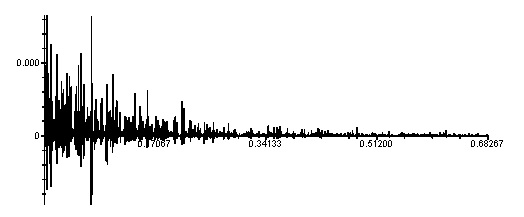
\includegraphics[width=7.6cm]{fig2}
                    \caption{Respuesta al impulso registrada en el punto}
                    \centering
                \end{figure}